\chapter{Methodology}\label{ch:methodology}

\section{Datasets}

In this work, we use question-answering and image captioning tasks to analyze the representations of pretrained and fine-tuned LLaVA, benchmark performance, and run functional localization experiments of visual instruction following.

\subsection{Question Answering} \label{sec:question_answering}

To gain an understanding of how fine-tuning affects LLaVA, we benchmarked both the pretrained and fine-tuned models on standard text-based and visual (multimodal) question answering (QA) benchmarks (Figure \ref{fig:datasets_diagram}). Comparing their performance across modalities provides a first indication of how fine-tuning impacts LLaVA's ability to integrate image understanding into its overall capabilities.

\begin{figure}
  \centering
  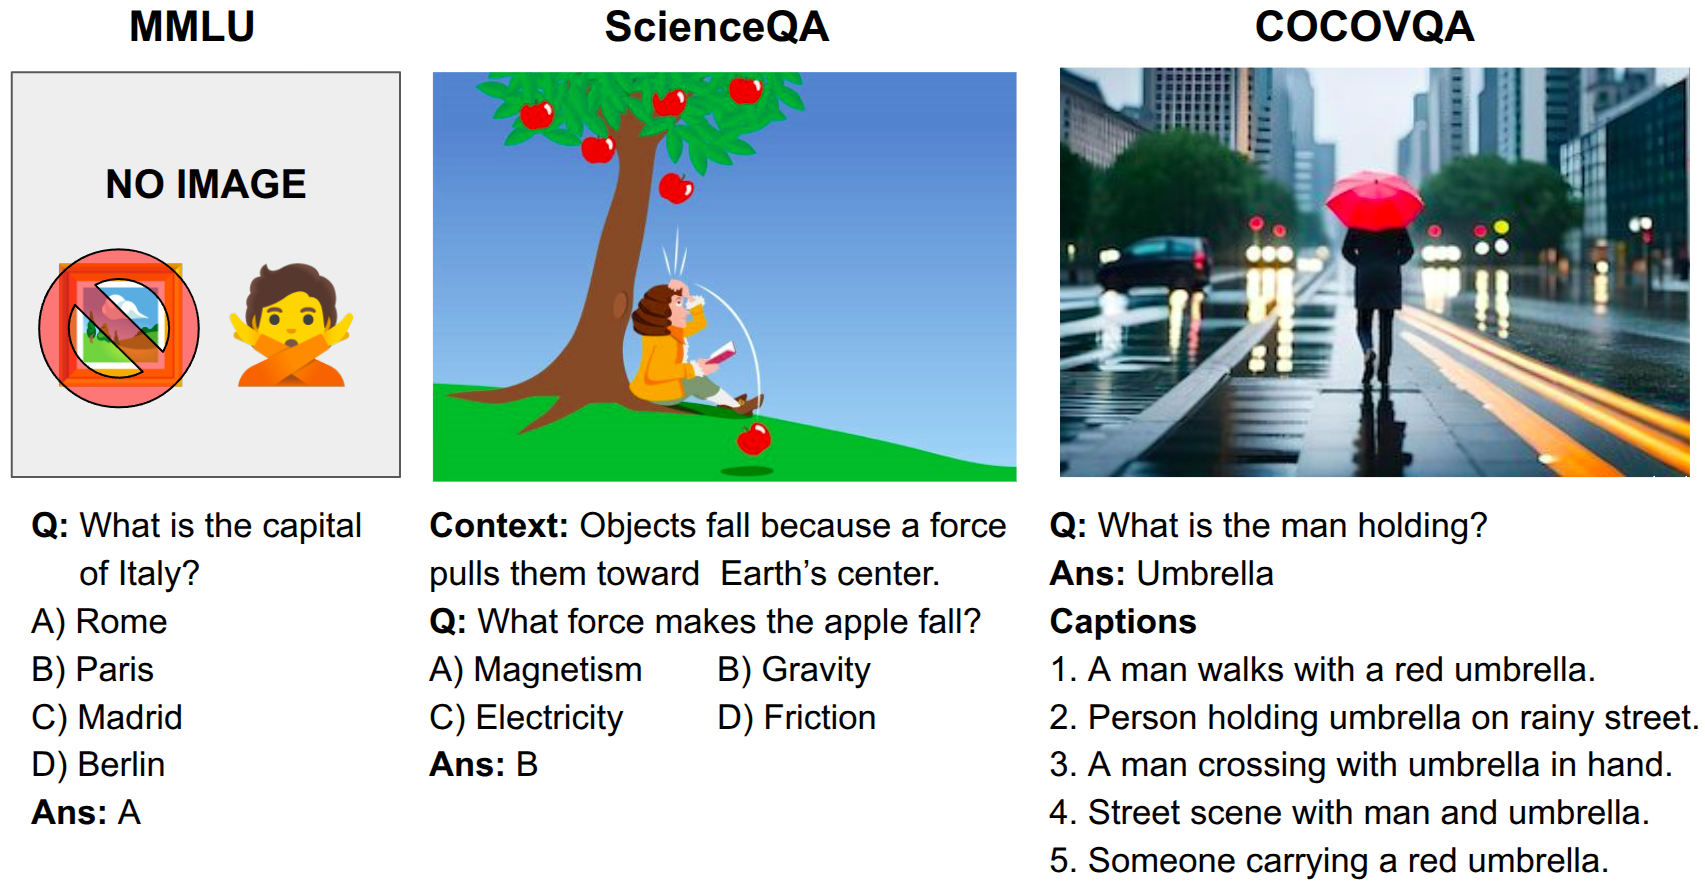
\includegraphics[width=\textwidth]{../images/chapter2/datasets_diagram.png}
  \caption{Benchmarks used in this study. (1) MMLU---text-only, multiple-choice QA; (2) ScienceQA---multiple-choice QA with optional text and/or image context; (3) COCOVQA---open-ended (single-word) QA built from COCO/COCOQA, with matched image and caption variants for the same items.}
  \label{fig:datasets_diagram}
\end{figure}

\paragraph{MMLU.}

The Massive Multitask Language Understanding benchmark (MMLU) \cite{hendrycksMeasuringMassiveMultitask2021} is widely used to test factual knowledge across diverse academic and professional fields in state-of-the-art LLMs \cite{touvronLlama2Open2023, wangHowFarCan2023, teamGemma3Technical2025}. It is purely text-based, consisting of multiple-choice questions grouped into subjects (e.g., history, physics, law). Each question provides only a stem and answer options, with no additional context. Although MMLU contains no images, it serves as a text-only baseline to anchor our results to widely reported LLM baselines. In this work, we used the Hugging Face implementation \href{https://huggingface.co/datasets/cais/mmlu}{\texttt{cais/mmlu}} \cite{mmlu_dataset}.

\paragraph{ScienceQA.}

The ScienceQA dataset \cite{luLearnExplainMultimodal2022} extends QA into the multimodal domain and is one of the benchmarks used to train and evaluate LLaVA models \cite{liuVisualInstructionTuning2023, liuImprovedBaselinesVisual2024, liLLaVANeXTInterleaveTacklingMultiimage2024, zhangLLaVAMiniEfficientImage2025}. Each question includes a stem and answer choices, along with optional supporting context (text and/or an image). Unlike MMLU, which never provides context, ScienceQA includes it. Importantly, if a ScienceQA item contains an image, there is no paired version where the same question is provided with a textual description of the image. For this study, we used the Hugging Face implementation \href{https://huggingface.co/datasets/yerevann/coco-karpathy}{\texttt{yerevann/coco-karpathy}} from Huggingface \cite{coco_karpathy_dataset}.

\paragraph{Custom Dataset: COCOVQA.}

While ScienceQA allows comparison across modalities, its multimodal questions do not have textual equivalents with identical content. To enable direct comparison on the same task and content but different modalities, we constructed a custom benchmark by combining COCO \cite{linMicrosoftCOCOCommon2015} and COCOQA \cite{renExploringModelsData2015}. COCO contains images with multiple captions but no questions, whereas COCOQA provides images (sourced from COCO) with questions and single-word answers but no captions.

Since COCOQA questions are linked to COCO images, we merged both datasets to create a unified set where each image is paired with captions, questions, and single-word answers. This allows evaluation under equivalent conditions in both text-based and visual QA. Unlike ScienceQA, here any given question can be answered either by looking at the image or by reading the caption, the latter often being easier for language models. This makes COCOVQA a more rigorous benchmark for comparing performance across modalities.

Specifically, we used the ``rest of validation set'' (\texttt{restval}) split of COCO from the Hugging Face dataset repository \href{https://huggingface.co/datasets/yerevann/coco-karpathy}{\texttt{yerevann/coco-karpathy}}---that implements the Karpathy splits for COCO \cite{karpathyDeepVisualSemanticAlignments2015}---and the ``test'' set of COCOQA from the Hugging Face dataset repository \href{https://huggingface.co/datasets/ThucPDCocoqaviDatasets}{\texttt{ThucPD/coco-qa-vi}} \cite{coco_qa_vi_dataset}. To avoid multiple QA samples per image during evaluation, we randomly selected one question-answer pair for each image. We refer to this combined dataset as COCOVQA, to distinguish it from COCOQA.

\paragraph{Evaluation Metric.}

Following the response format prompt for evaluation in \cite{liuImprovedBaselinesVisual2024} we prompted the models to \textit{answer the question with a single word or phrase} and formatted the prompt using the chat template of the model. Since the pretrained and fine-tuned models are chat models this makes the inputs to the models match the statistical patterns learned during fine-tuning for next-token prediction and thus makes the models evaluation more robust \cite{heDoesPromptFormatting2024, weiChainofThoughtPromptingElicits2023}. Testing without this formatting degraded performance, particularly the pretrained model, confirming the importance of using response-format prompts aligned with training distributions.

All the question answering tasks used zero-shot evaluation. The benchmarks evaluated here are multiple-choice questions, where the answers are one character in the case of MMLU and ScienceQA (A, B, C, D, E) or open-ended questions, where the answers are a single word in a finite set of words, which is the case of COCOVQA. The metric for these kind of datasets in the literature is exact match accuracy, either directly for multiple-choice questions or after a preprocessing step for open-ended questions \cite{renExploringModelsData2015, luHierarchicalQuestionImageCoAttention2017, liuImprovedBaselinesVisual2024}.

For the multiple-choice questions we made the models generate a single token and for the open-ended questions a maximum of $10$ tokens. The latter is a trade-off between not letting the model generate too much text that could end up getting it right by chance and the fact that the model should be able to generate a single word or phrase as instructed. We used up to $N=2500$ samples for evaluation purposes for reasons explained in Section \ref{sec:no}.

\subsection{Image Captioning} \label{sec:image_captioning}

For image captioning we use the COCOVQA images and instruct the model to produce a single-sentence caption with the following prompt:

{\small
\begin{verbatim}
  "Please look carefully at this image and provide a short, descriptive caption. "
  "Focus on the main objects, actions, and scene elements. "
  "Keep the caption concise but informative, similar to how you would describe "
  "the image to someone who cannot see it. "
  "Be specific about what you see without being overly detailed. "
  "THE CAPTION SHOULD BE A SINGLE SENTENCE, NOT MULTIPLE SENTENCES!!!"
\end{verbatim}
}

The instruction is wrapped with the model's chat template for consistency with training-time input format. We set the maximum generation length to 100 tokens to verify instruction-following (single-sentence constraint) without truncating valid outputs.

\noindent\textbf{Evaluation Metrics}

We evaluated generated captions with two complementary metrics:

\paragraph{CIDEr.}
The Consensus-based Image Description Evaluation (CIDEr) metric \cite{vedantamCIDErConsensusbasedImage2015} measures how closely a machine-generated caption matches what most humans would say about the image, i.e.,  its ``consensus''. It converts both the candidate caption and multiple human-provided references into vectors of n-grams, weighting each n-gram by Term Frequency-Inverse Document Frequency (TF-IDF) to downplay too-common words and highlight informative ones. It then computes cosine similarity between the generated and reference vectors, effectively rewarding captions that echo the human consensus \cite{jeongTechnicalReportNICE2024}. CIDEr has been shown to correlate strongly with human judgment in image captioning tasks, particularly when multiple reference captions are available, making it a standard benchmark for evaluating image captioning systems.

\paragraph{CLIP-Score.}
The CLIP-Score \cite{hesselCLIPScoreReferencefreeEvaluation2022} is a reference-free evaluation metric for image captioning that leverages the multimodal CLIP model \cite{radfordLearningTransferableVisual2021} to measure the semantic alignment between a caption and its corresponding image. By encoding both the image and generated caption into a shared multimodal embedding space and computing their cosine similarity, the CLIP-Score quantifies how well the caption captures the image content at a high conceptual level, prioritizing visual-semantic consistency rather than surface-level text similarity \cite{hesselCLIPScoreReferencefreeEvaluation2022}. This approach is especially useful when reference captions are unavailable or insufficient, making CLIP-Score a principled and widely adopted tool for evaluating the fidelity of image-to-text generation tasks.

\section{Residual Stream Extraction Method}\label{sec:residual_stream_extraction_method}

Representational similarity analyses of neural networks such as transformer models requires extracting the residual stream representations of a dataset. Figure \ref{fig:transformer_decoder_block} shows a LLaMA-style decoder block and the tap points used for residual stream extraction in this work. To make these tap points precise, we first review how attention is implemented in transformers.

In transformer models, attention is implemented as multi-head attention \cite{vaswaniAttentionAllYou2023}:

\begin{equation}
\mathrm{MultiHead}(Q,K,V)=\mathrm{Concat}(\text{head}_1,\ldots,\text{head}_H)\,W^O,
\end{equation}

where $\text{head}_i=\mathrm{Attention}(QW^Q_i,KW^K_i,VW^V_i)$, $W^Q_i,W^K_i,W^V_i\in\mathbb{R}^{d\times d_k}$ are the per-head projections, and $W^O\in\mathbb{R}^{H d_k\times d}$ is the output projection matrix. Here $H$ is the number of heads and $d = H d_k$ is the model dimension. In a decoder block, masked self-attention is used to ensure causal language modeling, so $Q = K = V = x$ (after normalization).

The contribution of each head to the residual stream is:

\begin{equation}
\text{head\_proj}_i = \text{head}_i W^O_i
\label{eq:head_proj}
\end{equation}

where $\text{head}_i \in \mathbb{R}^{T\times d_k}$, $W^O_i\in\mathbb{R}^{d_k\times d}$, hence $\text{head\_proj}_i\in\mathbb{R}^{T\times d}$.


In our experiments, for every layer of the pretrained and fine-tuned LLaVA's LLM-backbones we recorded (Figure \ref{fig:transformer_decoder_block}):
\begin{enumerate}
    \item the per-head attention output projection $\text{head\_proj}_i$ (Eq. \ref{eq:head_proj}), before the residual connection; and
    \item the output of the decoder layer.
\end{enumerate}

In decoder-only transformers, the last token in the sequence is the most contextualized and, in the final layer, feeds the next-token logits. Following prior work on transformers interpretability \cite{doimoRepresentationLandscapeFewShot, serraNarrowGateLocalizeda, valerianiGeometryHiddenRepresentations2023}, we use the last-token embedding as the sequence's representative in most experiments. Thus, for each input, a single $d$-dimensional vector is extracted at each tap point for analysis. Unless stated otherwise, all analyses in this work use the residual stream at each layer output.

\begin{figure}
\centering
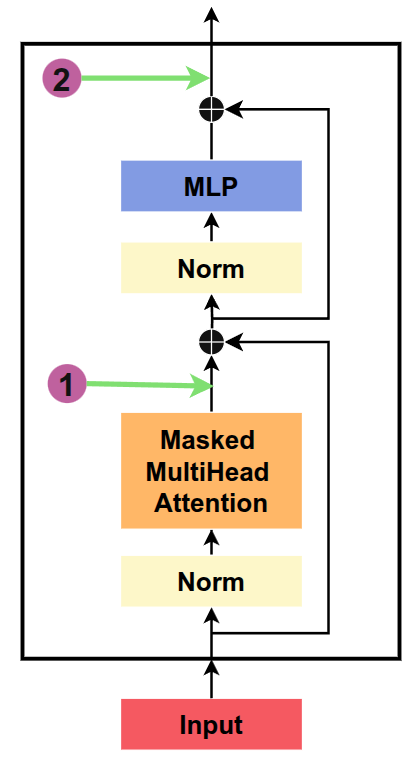
\includegraphics[width=0.25\textwidth]{../images/chapter2/transformer_decoder_block.png}
\caption{
  LLaMA-style pre-norm decoder block and the two tap points for the residual stream extraction:
  \textbf{(1)} per-head attention projection after $W^O$ (pre-residual connection),
  \textbf{(2)} output of the decoder layer.
}
\label{fig:transformer_decoder_block}
\end{figure}

For implementation, we used Hugging Face checkpoints of \href{https://huggingface.co/llava-hf/llava-1.5-7b-hf}{LLaVA-v1.5-7B} \cite{liuImprovedBaselinesVisual2024} and \href{https://huggingface.co/lmsys/vicuna-7b-v1.5}{Vicuna-v1.5-7B} \cite{zhengJudgingLLMasaJudgeMTBench}. To instantiate the pretrained LLaVA setting, we pair the Vicuna-v1.5-7B backbone with the released \href{https://huggingface.co/liuhaotian/llava-v1.5-mlp2x-336px-pretrain-vicuna-7b-v1.5}{pretrained MLP connector} \cite{liuImprovedBaselinesVisual2024} and kept the rest of the model architecture unchanged (see Figure~\ref{fig:llava_architecture}; Section~\ref{sec:llava}); the fine-tuned LLaVA is the public instruction-tuned checkpoint.

\section{Representational Similarity Measures}\label{sec:similarity_measures}

To examine how fine-tuning alters the internal geometry of LLaVA, we compared the pretrained and fine-tuned models using established measures of representational similarity. Given two sets of representations $X \in \mathbb{R}^{N \times d}$ and $Y \in \mathbb{R}^{N \times d'}$ extracted from the same dataset, these methods quantify the degree to which the two sets encode similar information \cite{klabundeSimilarityNeuralNetwork2025}. In our case, $X$ and $Y$ correspond to the residual stream embeddings of the last token across inputs, obtained from different LLaVA checkpoints.

We focus on two methods (Neighborhood Overlap and Linear CKA) that have proven effective for analyzing representation similarity in deep neural networks, particularly transformers \cite{doimoHierarchicalNucleationDeep2020, basileIntrinsicDimensionCorrelation2025, kornblithSimilarityNeuralNetwork2019}.

\subsection{Neighborhood Overlap}\label{sec:no}

Neighborhood Overlap (NO) measures how much of the local geometry of the representation space is preserved between two sets of embeddings through the nearest neighbors of each data point \cite{doimoHierarchicalNucleationDeep2020,klabundeSimilarityNeuralNetwork2025}. For each sample, it compares the $k$-nearest neighbors ---measured with respect to a distance metric--- in $X$ with those in $Y$ and computes the fraction of overlap:

\begin{equation*}
    \text{NO}(X,Y) = \frac{1}{Nk} \sum_{i=1}^{N} |\mathcal{N}_k(X_i) \cap \mathcal{N}_k(Y_i)|
    \label{eq:no}
\end{equation*}

where $\mathcal{N}_k(X_i)$ denotes the set of $k$ nearest neighbors of sample $X_i \in \mathbb{R}^d$. By definition, $\text{NO}(X,Y) \in [0,1]$, with higher values indicating stronger preservation of local structure between the two representation spaces.

In our experiments, we used the Euclidean distance as the distance metric and set $k=30$, following prior work showing this value sufficiently captures structural similarity in neural networks in a similar setting \cite{doimoHierarchicalNucleationDeep2020, doimoRepresentationLandscapeFewShot, serraNarrowGateLocalizeda}. To balance accuracy and computational cost, we fixed the maximum number of samples to $N=2500$, consistent with the scale used in earlier studies.

\subsection{Linear CKA}

Linear Centered Kernel Alignment (CKA) \cite{kornblithSimilarityNeuralNetwork2019, davariReliabilityCKASimilarity2022, klabundeSimilarityNeuralNetwork2025} is a measure of the degree of linear correlation between two representation spaces, which is invariant to isotropic scaling and orthogonal transformations. It is a normalized version of the Hilbert-Schmidt Independence Criterion (HSIC) \cite{grettonMeasuringStatisticalDependence2005}, which relies on the kernel trick to detect non-linear dependence between two variables, and was introduced to the deep learning context by \cite{kornblithSimilarityNeuralNetwork2019}. It has been shown to perform comparably to RBF-based CKA while being computationally efficient as it directly uses feature-space dot products. It is computed as follows:

\begin{equation*}
    \text{CKA}(X,Y) = \frac{\|Y^\top X\|_F^2}{\|X^\top X\|_F \cdot \|Y^\top Y\|_F}
    \label{eq:cka}
\end{equation*}

where $\| \cdot \|_F$ denotes the Frobenius norm. We can clearly see that it quantifies the linear correlation between the two spaces by summing the squared covariances between every pair of features across the two spaces. Due to the normalization of the self-similarities the influence of scaling is removed and $\text{CKA}(X,Y) \in [0,1]$.

\section{Geometry of Representations}

\subsection{Intrinsic Dimension of Representations}\label{sec:id}

To complement similarity-based analyses, we also examined how fine-tuning changes the geometric complexity of LLaVA's internal representations by estimating their intrinsic dimension (ID). Whereas similarity measures capture overlap between pretrained and fine-tuned checkpoints, ID provides a different perspective: it quantifies whether fine-tuning makes the representation manifold more compact, more redundant, or more expressive.

Formally, the intrinsic dimension of a dataset is the minimum number of degrees of freedom required to locally describe its data manifold \cite{ansuiniIntrinsicDimensionData2019}. In this work, the ID of each representation matrix $X \in \mathbb{R}^{N \times d}$ was estimated using the Generalized Ratios Intrinsic Dimension Estimator (Gride) \cite{dentiGeneralizedRatiosIntrinsic2022}, an extension of the two-nearest-neighbor (2NN) method \cite{faccoEstimatingIntrinsicDimension2017}. Gride builds on the result that, when data points lie on a smooth manifold of dimension $\delta$ with constant density, the ratio between distances to successive neighbors follows a distribution that depends only on $\delta$ \cite{faccoEstimatingIntrinsicDimension2017,dentiGeneralizedRatiosIntrinsic2022}.

For a given point $X_i \in \mathbb{R}^d$, Gride generalizes the computation of the intrinsic dimension to arbitrary neighbor ranks $k_1$ and $k_2$, with distances $r_{i,k_1}$ and $r_{i,k_2}$, with respect to a distance metric. In the original 2NN estimator \cite{faccoEstimatingIntrinsicDimension2017}, these ranks were fixed at $k_1 = 1$ and $k_2 = 2$. A common choice in Gride \cite{dentiGeneralizedRatiosIntrinsic2022, doimoRepresentationLandscapeFewShot} is $k_1 = k$ and $k_2 = 2k$, where $k$ is the base neighbor rank. This generalization enables multi-scale analysis and reduces bias that may arise at very small scales. The distance ratio $\mu_k = \frac{r_{i,k_2}}{r_{i,k_1}}$ is then used to fit a maximum likelihood model of the form \cite{dentiGeneralizedRatiosIntrinsic2022}:

\begin{equation*}
\mathcal{L}(\delta) \propto \delta (\mu_k^{\delta} - 1)^{k-1}  \mu_k^{(1-2k) \delta - 1} \; , \; \mu_k > 1
\label{eq:gride_likelihood}
\end{equation*}

whose maximizer yields the ID estimate at the chosen neighbor scale.

Although the method assumes constant density, it has been shown to remain robust as long as density is approximately constant over the relevant neighborhood \cite{dentiGeneralizedRatiosIntrinsic2022}. In this work, we followed prior studies \cite{doimoHierarchicalNucleationDeep2020, doimoRepresentationLandscapeFewShot, serraNarrowGateLocalizeda} and used $k = 16$, corresponding to neighbor ranks $k_1 = 16$ and $k_2 = 32$, with Euclidean distance as the metric. All computations were performed using the \href{https://dadapy.readthedocs.io/en/latest/}{\texttt{Dadapy}} library \cite{glielmoDADApyDistancebasedAnalysis2022}.

\subsection{Modality Gap}

\paragraph{Experiment Setup.} \label{sec:modality_gap_experiment_setup}

To evaluate how fine-tuning reshapes LLaVA's backbone representations, we examined the \emph{modality gap}---the geometric separation between text and image embeddings. This analysis indicates whether fine-tuning promotes tighter integration between modalities or preserves their separation.

Unlike CLIP---which uses separate encoders and returns individual global embeddings for text and for images---LLaVA is a decoder model that encodes both modalities in a shared representational space and does not yield a single, fixed embedding per modality. Therefore, representative embeddings for each modality must be constructed in a task-specific way. Using solely the last embedding in a sequence as in Section~\ref{sec:residual_stream_extraction_method} might not be suitable to fully represent textual and visual information from the inputs because although this embedding is the most contextualized, it also contains the information for the next token prediction, which might bias the representation. 

In this work, we extracted text and image embeddings from image QA and image captioning tasks using the COCOVQA dataset. The core idea is to control the order of text and image input content so that the modality placed last is the most contextualized; we then select a representative from those embeddings. Concretely, we \emph{randomly choose one embedding per sample}, which might mitigate next-token bias while preserving the modality's contextual information.

By default, LLaVA's chat template places image embeddings before text embeddings. For QA, the structure of the prompt is:

\begin{verbatim}
<SYSTEM MESSAGE>
USER: <IMAGE> 
<QUESTION>
Answer the question with a single word or phrase.
ASSISTANT: Answer:
\end{verbatim}

where \texttt{<SYSTEM MESSAGE>}, \texttt{<IMAGE>}, and \texttt{<QUESTION>} are placeholders for the system message, image, and question about the image. Here, \texttt{<IMAGE>} is a special token replaced by image embeddings after tokenization. The only thing the chat template does is to structure the multiple input contents (e.g., system message, image, and question in this case) into a single string that forms the conversation between the \texttt{USER} and \texttt{ASSISTANT}, ensuring compatibility with the model's instruction-following behavior.

In this setup, text tokens appear at the end and are therefore the most contextualized. For each sample, we randomly select one text embedding to represent the textual modality, focusing in the embeddings of the question.

To make image embeddings maximally contextualized, we manually reversed the input order so that text comes before the image, as in:

\begin{verbatim} <SYSTEM MESSAGE>
USER: <QUESTION> <IMAGE>
Answer the question with a single word or phrase.
ASSISTANT: Answer:
\end{verbatim}

In this case, we randomly select one of the image embeddings for each sample.

A similar setup was used for image captioning. To enrich the context, we provided the model with the ground-truth captions and asked it to generate an additional description. Unlike the captioning setup in Section \ref{sec:image_captioning}, here the task is to extend existing captions rather than generate one from scratch. The prompt looks like:

\begin{verbatim} <SYSTEM MESSAGE>
USER: <IMAGE>
Below are 5 numbered descriptions of the image.
Please generate an additional description of the image.
The caption should be a single sentence, not multiple sentences!!!

1. <CAPTION 1>
2. <CAPTION 2>
3. <CAPTION 3>
4. <CAPTION 4>
5. <CAPTION 5>

ASSISTANT: Answer:
\end{verbatim}

From these tasks, we obtained two matrices, $X_{\text{text}}, X_{\text{image}} \in \mathbb{R}^{N \times d}$, where $N$ is the number of samples and $d$ the representation dimension. We then computed two measures:

\begin{enumerate}
    \item Median cosine similarity (input-wise): captures the directional alignment of text vs. image embeddings in high-dimensional space. Importantly, embeddings may align directionally yet still form separate modality-specific clusters \cite{liangMindGapUnderstanding2022,roleFillGapQuantifying2025}.
    \item Homogeneity score after clustering: using the Advanced Density Peaks (ADP) clustering algorithm \cite{derricoAutomaticTopographyHighdimensional2021}, we evaluated whether embeddings form distinct clusters by modality. The homogeneity score \cite{rosenbergVMeasureConditionalEntropyBased} quantifies this separation.
\end{enumerate}

Together, these measures provide complementary perspectives: cosine similarity captures cross-modal alignment, while clustering-based homogeneity reveals whether text and image embeddings remain segregated in representational space. This follows the methodology of Serra et al. \cite{serraNarrowGateLocalizeda}, who examined modality gaps across different VLMs, including LLaVA. Together, these measures allow us to test whether visual instruction tuning reduces the modality gap or preserves their separation, thus providing concrete evidence of how fine-tuning reshapes the internal geometry of LLaVA's representations.

Because cosine similarity is a widely known metric, here it is not described further; instead, the Advanced Density Peaks (ADP) clustering algorithm, which underlies the cluster structure used in this analysis, is described next, followed by the homogeneity score that quantifies cluster purity. Together, these sections connect the experimental setup with the clustering-based evaluation of the modality gap.

\paragraph{Advanced Density Peaks (ADP) Clustering.}

ADP clustering \cite{derricoAutomaticTopographyHighdimensional2021} is a non-parametric density-based clustering algorithm that automatically determines the optimal number of clusters by identifying statistically significant density peaks in high-dimensional datasets. The algorithm operates on the fundamental principle that cluster centers correspond to local density maxima in the data manifold, while clusters are naturally separated by regions of lower density. 

The method follows a three-stage process. First, it estimates the local density $\rho_i$ of each data point $X_i$ using a k-nearest neighbor approach, computing both density values and their statistical uncertainties $\varepsilon_i$. The local densities $\rho_{i, k} = \frac{k}{N V(r_{k}, \delta)}$ are estimated on the intrinsic manifold, where $V(r_{k}, \delta)$ is the volume of the $k$-dimensional sphere of radius $r_{k}$ in a $d$-dimensional space with intrinsic dimension $\delta$. The algorithm then identifies putative cluster centers as points that represent local density maxima within their k-nearest neighbor regions. Each remaining point is then preliminarily assigned to its nearest density peak based on density gradients toward higher-density regions. Finally, for each peak, the algorithm considers the saddle point shared with another peak, with density $\rho_{c, c'}$ and uncertainty $\varepsilon_{c, c'}$. It computes the standardized density drop test statistic: 

$$
T = \frac{\log\rho_{c} - \log\rho_{c, c'}}{\varepsilon_{c} + \varepsilon_{c, c'}},
$$

where $\rho_{c}$ and $\varepsilon_{c}$ are the density of the peak of the cluster $c$ and uncertainty of the peak density, respectively. If this value does not exceed a predefined Z-score confidence threshold, the two peaks are merged. This merging step is applied iteratively until only clusters supported by statistically significant peaks remain.

In this work, the local density of each point is computed with a fixed $k$-nearest neighbor estimator ($k=16$), following established practices in representation analysis \cite{doimoHierarchicalNucleationDeep2020, doimoRepresentationLandscapeFewShot, serraNarrowGateLocalizeda} as it has been shown to work better for representations of neural networks, rather than using point-adaptive density estimation methods \cite{derricoAutomaticTopographyHighdimensional2021}. The intrinsic dimension of the data representation is first estimated with the Gride algorithm (Section~\ref{sec:id}) using the Cosine distance, and this value is used in the density computation. The confidence threshold for merging peaks was set to $Z=1.65$, corresponding to $95\%$ one-tailed confidence in a $Z$-test. For clustering the image and text embeddings together their extracted representation matrices are concatenated into a $2N\times d$ matrix. All ADP clustering steps are performed using the \texttt{Dadapy} library. The algorithm returns the cluster labels for each point.

The clustering performance is evaluated using the homogeneity score, a clustering validation metric that measures whether each cluster contains only members of a single class \cite{rosenbergVMeasureConditionalEntropyBased}. The homogeneity score is computed as $h = 1 - H(C|K)/H(C)$, where $H(C|K)$ represents the conditional entropy of class distribution $C$ given the cluster assignment $K$ and $H(C)$ is the entropy of the overall class distribution. This metric ranges from $0$ to $1$, where a score of $1$ indicates perfect homogeneity (each cluster contains samples from exactly one class, so knowing the cluster assignment completely determines the class label and leaves no uncertainty about it) and $0$ represents the worst case scenario where class distributions within clusters are completely mixed, so the cluster assignment gives no information about the class.

% (each cluster contains samples from only one class, so the cluster label uniquely determines the class label)


% and a score of 0 indicates complete lack of homogeneity (the class distribution inside each cluster is identical to the overall class distribution, so knowing the cluster assignment gives no information about the class label).

\section{Functional Localization via Layer Patching}\label{sec:functional_localization_via_layer_patching}

We test whether the capabilities gained through visual instruction tuning are \emph{localized} to specific backbone layers or \emph{distributed} across the network. To do so, we conducted \emph{layer patching} experiments: layers from the fine-tuned LLaVA backbone are inserted into the pretrained backbone either (i) cumulatively from the input to the output of the network, or (ii) in a sliding window fashion that replaces only a contiguous subset at a time. Performance differences across tasks indicate where the fine-tuned functionalities emerge. The tasks used for these experiments are question answering and image captioning.

Only the subset of LLM backbone layers being tested changes between runs; the vision encoder and connector remain fixed, and the LM head is kept unless explicitly stated.

\paragraph{Question Answering.}
We evaluate exclusively on the COCOVQA dataset to enable controlled, like-for-like comparisons across modalities with identical content. For each configuration (cumulative or sliding-window), we replace a specified set of pretrained backbone layers with their fine-tuned counterparts and measure zero-shot accuracy under the same prompting and formatting used in Section~\ref{sec:question_answering}.

The rationale is that by holding the task and input distribution fixed while varying which layers are patched, we isolate which layers in the fine-tuned backbone contribute the most to multimodal QA, and whether improvements accumulate across layers or hinge on a few critical ones.

\paragraph{Image Captioning.}
The image captioning setup is the same as in Section~\ref{sec:image_captioning}.

\section{Computational Resources and Reproducibility}

All our experiments ran on a single NVIDIA A100 (40 GB) GPU on the ORFEO cluster of AREA Science Park. To promote determinism and reproducibility, we fixed the random seed to \texttt{42} and disabled PyTorch stochasticity. For all model generations we used greedy decoding, which in Huggingface is implemented as \texttt{generate(..., do\_sample = False)}. All models were loaded in \texttt{fp16} (half-precision).